
What is software engineering for AI systems? What kind of AI do we want for SE applications? If we look into
 the literature, we can see two at least  two different views on this issue:
 \bi
 \item Software 2.0
 \item ML-as-requirements engineering
 \ei
 
  
 In the AI literature, formal descriptions of explanation
 often assert that minimality is a necessary precondition for ``good'' explanations.


Poole's THEORIST system~\cite{Poole1994WhoCT} offers a clean logical framework of such reasoning.
In that framework, a goal graph is a  {\em theory} that contains a small number of upper-most {\em goals}. When we reason about that theory, we make {\em assumptions}
about either (a)~initial facts or (b)~how to resolve contradictory decisions. In the general case, only some subset of the theory can be used to achieve some of the goals using some of the assumptions without
leading to contradictions (denoted $\bot$). That is:


    {\small \begin{equation}\label{eq:subs}
     \begin{array}{r@{~}c@{~}l}
       T &\subseteq& \mathit{theory} \\
       A &\subseteq& \mathit{assumptions}\\    
       G &\subseteq& \mathit{goals}\\
       T \wedge A&  \vdash & G\\
       T \wedge A & \not\vdash& \bot
       \end{array}
     \end{equation}}
     A {\em world of belief} is a solution that
     satisfies these invariants.
     For many years we have tried to find such worlds using a variety of
     methods. For example Menzies' HT4 system~\cite{menzies1996applications}
     combined forward and backward chaining to generate worlds while Ernst \etal~\cite{ernst12caise} used DeKleer's ATMS (assumption-based truth-maintenance system)~\cite{de1986assumption}.
Those implementations suffered
from cripplingly slow runtimes that scaled very poorly to larger models. Such slow runtimes are not merely a quirk of those implementations---rather they are fundamental to the process of exploring models with many contradictions.
It is easy to see why:
exploring all the subsets in Equation~\ref{eq:subs} is a very slow process.
     Bylander \etal~\cite{Bylander1991}  and
     Abdelbar \etal~\cite{Abdelbar:2004} both confirm that abduction is NP-hard;
     i.e. when exploring all options within a requirements goal model, we should expect very slow runtimes.


Formal  descriptions of ``explanation'' date back to Aristile's 4th figure. 


Explanation is often d
 
 As to examples of how-to-change AI systems, perhaps the most famous is LIME~\cite{ribeiro2016should}
 from KDD 2016.
 For another example, Peters'
 counterfactual generator~\cite{peters2015lace2} (the search for the delta between some current situation and the nearest
 neighbor of a different class) can be read as a least-effort
 recommended plan  on how to adjust the classification 
 of an instance. For a detailed list of other AI explanation systems that report how to change a system, see {\S}2.1 of Shokri et al.~\ref{shokri2021}.

  
  
 convincingly that AI researchers have confused 
 
Apart from Rubin, 
 
 
 To begin with, we need some workable definitions of explanation. The AI community has yet to reach an agreement on those definitions.
A recent systematic literature review by Violane et al. ~\cite{vilone2020explainable} finds that the AI literature connects many terms to ``explanation'' to summarize the field of AI and explanation.
Their Table1 lists 37 terms that, in the literature, are related to explanation\footnote{
Algorithmic transparency, 
actionability, 
causality, 
completeness, 
comprehensibility, 
cognitive, 
correctability, 
effectiveness, 
efficiency, 
explicability, 
explicitness, 
faithfulness, 
intelligibility, 
interactivity, 
interestingness, 
interpretability, 
informativeness, 
justifiability, 
mental fit, 
monotonicity, 
persuasiveness, 
predictability, 
reversibility, 
robustness, 
satisfaction, 
scrutability / diagnosis, 
security, 
selection/simplicity, 
sensitivity, 
simplification, 
soundness, 
stability, 
transparency, 
transferability and, 
understandability}. Despite the length of this list, it is incomplete. For example,
that review does not cover the 
misses key concepts.
For example, 
 Vilone and Longo   do not reflect on
how explanations can be discriminate against different social groups. This omission is interesting
since when 
  



Another lesson from  Table~\ref{words} is that there is much variance in how
professional, industrial, and
governmental organizations approach issues of explanation and fairness and AI.
 Many researchers have commented on this
variability.
In  a very widely cited paper\footnote{2251 citations, as of Jul 2021.}, 
Lipton~\cite{lipton2018mythos} laments that there is little
agreement on what   
  ``interpretability'' means
  (and how to assess it) within the
 the machine learning community. 
 In a somewhat more detailed analysis than Lipton,
 Broniatowski~\cite{Broniatowski21} argues
 convincingly that AI researchers have confused:

 
 One myth   mentioned
 by Lipton is that   models are ``interpretable'' if they are 
 symbolic in nature and succinct 
 (i.e. humans can read them, very quickly).
The following example  (used later in this proposal)
illustrate how a succinct symbolic model is not necessary readily explainable.
K\"astner~\cite{kastner21} argues that ``sparse linear models'' are ``intrinsically interpretable'' but that
 claim is debatable\footnote{Here, we are not saying
 that K\"astner is in error. Rather, we are saying
 that he is offering commentary on a highly evolving field where the core terms are undergoing 
 continual refinement}. 
 Suppose an analyst wants an explanation
 of what is a ``fuel efficient lightweight car with good acceleration''. The file
{\em auto93} (from the UC Irvine ML
  repository) has hundreds of examples of cars that mention those features as well as the number of cylinders $c$, horsepower $h$, 
displacement $d$ (a.k.a. size of car), year of release $y$ and country of origin $o$.
Using linear regression, we can learn learn the model of Equation~\ref{one}.
 
 
\begin{wrapfigure}{r}{3in}
{\footnotesize
\begin{equation}\label{one}
\begin{array}{r@{=}l} 
  \mathit{weight} &
 60.7{\times}c +
      5.2{\times}d +
      4.1{\times}h +
     13.7{\times}y +
    -48{\times}o +
    234.2 \\     
  \mathit{mpg} &
     -0.6{\times}c +
     -0.1{\times}d +
     -0.1h +
      0.6{\times}y +
      1.2{\times}o +
     -12.9 \\   
 \mathit{accel} &
      0.1{\times}c +
      0.1{\times}d +
     -0.1h +
      0.1{\times}y +
     -0.2{\times}o +
     21.2\end{array} \end{equation}
     }
  \end{wrapfigure} 
   
  Equation~\ref{one}  can be used
  to assess the impact of design decisions
  on the disjunction of 
    weight {\em or} mph  {\em or}  acceleration.
    But if we wanted to reason about
    the conjunction
    (of
     weight {\em and} mph  {\em and}  acceleration).
 Generation 
(about what is a  ``fuel efficient lightweight car with good acceleration'').
Such an explanation must trade-off between the completing concerns
of weight, mpg and acceleration. This can be a
surprisingly complicated process.
For example, NSGA-II is a standard tool for
multi-goal optimization that  could
(a)~mutate population of cars,   (b)~scores the mutants
on the above three equations, then (c)~select the best scoring mutants as parents for
the next generation of mutants.
That genetic algorithm approach may not scale to large problems.
For example, starting with equations not much more complex than Equation~\ref{one},
PI Menzies and his graduate student
Kewen Peng~\cite{kewen21} applied
NSGA-II to explore $C=10^4$ software configuration options
(in order to optimize for $G=2$ goals). In that application,
the $O(GC^3)$ non-dominating sort procedure of the NSGA-II~\cite{deb02}   took hours to terminate.  

(Technical aside: later in this proposal,
the xPLAIN0 algorithm will offer a much faster
way to succinctly explain Equation~\ref{one}.)  

 






Since, experts post far fewer to-do's  in their STMs, they complete their tasks faster because (a) they are less encumbered by excessive reflection and (b) there is more space in their STM to reason about new information. 
First proposed in 1981, this   theory  still remains relevant
Humans best understand a model
which can ``fit'' it into their LTM; i.e., when that model comprises many small fragments.
Phillips et al.~\cite{phillips2017FFTrees} and others~\cite{gigerenzer2008heuristics,gigerenzer2011heuristic,czerlinski1999good} discuss how models containing tiny rule fragments can be  quickly comprehended by 
doctors in emergency rooms making rapid  decisions; or by soldiers on guard  making snap decisions about whether to fire or not on a potential enemy; or by  stockbrokers making instant decisions about buying or selling stock.
This theory-of-small-fragments explains both expert competency and incompetency in software
engineering tasks such as understanding code~\cite{Wi96}. 
Specifically,   expert-level comprehension means
having rules that   quickly lead to decisions, without clogging the STM.

 


This proposal will:
  
  \begin{center}
 {\bf Goal1: Test if the keys-based {\IT} approach     enables
          \underline{F}aster 
               anyt\underline{I}me 
                \underline{R}equirements 
                \underline{E}ngineering.
                }
 \end{center}
We call this ``requirements engineering''  
 since   Shaw~\cite{shaw1980becoming}, Kastner~\cite{kastner20}
 and Zimmermann~\cite{timzim13} argue that 
 AI tools  in SE is best seen as a  discovery process that uncovers
 what is possible. For that purpose,
 we want anytime
algorithms~\cite{zilberstein1996using} which, at anytime,
 can be paused and queried for an adequate solution
 (and,
 at any further time, such anytime algorithms can
 find  better solutions).
  
  
\begin{table*} 
{\small
\begin{tabular}{|p{.98\textwidth}|}\hline
 \rowcolor{blue!10}
   PI Menzies and Zimmerman~\cite{timzim13} characterize  software analytics 
as a search through a space of many possible questions to find a small
number of most productive queries. At each step of this process, some AI learners
are applied to find some model from some current version of the collected data.
%& 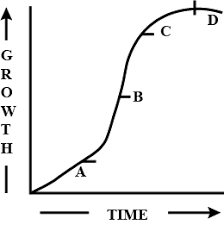
\includegraphics[width=2.25in]{fig/growth.png}
\\
 A similar process (where feedback from the AI guides future activity) is seen
in Briand's testing of cyberphysical systems~\cite{Abdessalem18} (in his case, the self-reversing systems
 of cars). In Briand's process, 
 \bi
 \item
 The current testing goals $G$ are used to collect new test
data $D$. 
\item
Neural nets  then synthesized that data  new features which decision
tree learners use to create new testing goals $G'$ (from the decision branches
  containing the most bugs). 
  \item
  These new testing goals are used
  to guides the collection
  of new data $D'$, at which point the cycle repeats (to generate $G''$ and  $D''$ and
  so on). 
  \item Note that at each step in the cycle, human engineers can lean in
  to see where the system is focusing the testing, as well as adjusting the proposed tests (using their domain knowledge).\ei\\
 \rowcolor{blue!10}
 Another relevant example here is the work of PI Menzies, Hu,Tu et al.~\cite{zhe19,tu20}: where
 humans quickly skim a few samples
looking for:
\bi
\item
Papers relevant to some research goal (using papers extracted from Google Scholar)
\item
or defect producing bugs (using  issues reports from Github projects) or (c) security
vulnerabilities (using code examples from Mozilla Firefox. 
\ei
In the active
learning approach of PI Menzies, Hu,Tu et al.~\cite{zhe19,tu20}:
\bi\item
Whenever a human finds an interesting paper/issue report, code sample,
then an AI tool updates an SVM model that tries to predict for ``that human would find this interesting''. 
\item
Once that model is working well, the human can relax and the AI can rush ahead to to find all the examples that matter to the human. 
\item
These auto-collected examples
can then be used to train a classifier for (a)~relevant papers, or (b)~defect-inducing
commits; or (c)~code with security vulnerabilities.
\ei\\\hline
\end{tabular}}
\caption{Examples of useful human + AI interaction in software engineering.}\label{interact}
\end{table*}

   
 
 \begin{table*} 
{\small
\begin{tabular}{|cccP{1in}p{4in}|}\hline
\rowcolor{blue!10}SE&2002 & \cite{DBLP:conf/re/FeatherM02} 
& NASA deep-space  missions &
In models with hundreds of options, controlling 30  was enough
to optimize for requirement functionality while minimizing risk and cost.\\
SE&2005 &\cite{DBLP:journals/software/ChenBMP05} &  Effort estimation  &
Best results   obtained after pruning 80\% of  features, or even more.\\
\rowcolor{blue!15}SE &2007 & \cite{DBLP:journals/tse/MenziesGF07} & Software quality \newline assurance
& In data sets with 40+ features, best defect predictors were built using 2 to 3 features.\\
SE&2017 & \cite{DBLP:conf/icse/MathewAM17} & Information needs for 
Com Sci departments & In iStar softgoals with hundreds of nodes and cross-node constraints, decisions on less than 12\%  of the nodes
was enough to minimize coast and maximize goal coverage.\\
\rowcolor{blue!10}SE& 2018  &\cite{chen2018sampling} & Software process models & Finding
optimal points within $N=10,000$ options
required just \mbox{$2*\log_2({N})$} evaluations, which implies that those
spaces are controlled by just $\log_2({2\log_2({N})})\approx 5$ features.\\
SE&2021 & \cite{agrawal2020simpler}& Stackoverflow  text mining& Within a space of $10^8$ possible parameter
settings for a learner, best results were achieved after evaluating just 30
options \\\hline
\rowcolor{blue!10}AI & 1986 &  \cite{amarel86} & Automated chess playing & After a search space expands, it then routinely collapses around a set of ``choke points'' that all solutions must traverse. Inference can be made faster by stepping faster between these
chock points. To say that another way,  the only features that mattered
where the  handful
of features found in the chock points.\\
AI & 1994 & \cite{Crawford94} & Scheduling & Local searches for better schedules quickly saturate (since so few features control ``better'').  Hence, the best way to repair a poor schedule is to abandon it  and jump far away in the search space.\\
\rowcolor{blue!10}AI & 1997&\cite{kohavi1997wrappers} & Feature subset\newline  selection & Models build from
$\sqrt{N}$ features (carefully chosen) performed as well or better than those
that use $N$ variables\\
AI & 2003 & \cite{Williams03} &  Backdoors to \newline theorem proving & After exhaustively  generating many solutions, it was seen that    solutions share a few  settings. If those settings are made {\em before} the next run, then subsequent inference becomes very fast.\\\hline
% \rowcolor{blue!10} other & 2010 & \cite{DBLP:journals/ase/GayMDG10} & Air traffic control &
% Genetic algorithms that took months of CPU and which explored 100,000s of variants
% were out-performed by tools that terminated in minutes, and only queried
% a very small number
% ($log_2{N}$) of  options.\\
% other & 2013 & \cite{partington15} & Community\newline nutrition &
% A modeling team was data 100s of data points from 300 supermarkets.
% It was shown that models that were just as effective could be built using just a handful of variables, collected from just 30 supermarkets.\\\hline
\end{tabular}}
\caption{Examples of the keys effect have been seen in many domains, from SE and elsewhere. In all
these examples, it has been observed that a few
key features control the rest.}\label{keysSE}
\end{table*}
  Given the 
   examples of Table~\ref{keysSE} (where entire systems
   were controlled, just by setting a few key variables), then our expectations for this keys-based approach are very high:
 {\bf   
 compared to the alternatives,
 keys-based reasoning should 
 \underline{reduce RE effort  by a factor
 of 10 to 100}.}
 Here by ``effort'' we mean  (a)~CPU time as well as 
 (b)~human time
spent on development and   maintenance. Also, by ``alternatives'',
we mean the  two obvious alternatives to  this keys-based proposal:
 interactive search-based software engineering (iSBSE)~\cite{ramirez2018systematic};
and sequential-model optimization (SMO)~\cite{hutter2011sequential}
 (for details on these two approaches, see   \S\ref{aa}).
 As shown in Table~\ref{casestudies}, there are many
such candidate case studies from the iSBSE and SMO literature. 
Hence,  we anticipate no problem with find case study material.

As shown in Table~\ref{keysSE}, our experience to date,
is that the keys effect is quite prevalent. Hence, it is worthy of
detailed that study. Nevertheless,
{\IT} will not work unless domain artifacts have a certain structure; i.e. 
a small number of features control the rest.  Accordingly, it is prudent 
to: 

\begin{center}
{\bf Goal2: Develop
detectors for the keys effect}  (since this  will tell us when
{\IT} should not be used). 
\end{center}
\noindent
When these two goals are achieved, this  work will deliver
   (a)~tools that   exploit  the  keys  effect  to dramatically
  reduce the effort required for using AI in SE; (b)~case  studies    documenting  the  comparative  benefits  (or  otherwise)  of  these tools; (c)~guidance on when to use, or when to avoid, those tools.
  
   
 
  
  
\begin{table}[!t]
  \caption{Case studies for this research.
  For details on how we will use these case studies within
  this proposal, see  \S\ref{howtest}. 
   }\label{casestudies}
{\small
\begin{tabular}{|p{.98\textwidth}|}\hline
 \rowcolor{blue!10} Our first case study will be 
 {\em humans exploring options in product lines}. The web site \url{splot-research.org} offers hundreds of such project lines in a machine-readable XML format. 
 Here, the
 {\bf requirements engineering problem} is to decide what features to support while minimizing development time, maximizing delivered
 functionality, while minimising expected number of bugs~\cite{Sayyad:2013:SPL,Sayyad:2013,henard2015combining}.\\
 
 Another case study will be
   {\em next-release planning} (NRP)~\cite{Aydemir18,pitangueira2017minimizing,Ameller17,dominguez2019efficient} where the 
 {\bf requirements engineering
 problem} is to rush out as much functionality as early as possible, while also taking time
 to build the libraries that simplify subsequent releases.
The literature includes numerous  NRP problems
 (e.g. see \url{github.com/MiguelAngelDominguezRios/anytime-nrp}).\\
 
\rowcolor{blue!10} Yet another case study will be {\em requirements
 engineering for software maintenance}.
 Given   code marked   with feature flags~\cite{parnin2017top,rahman2016feature}
 and project health indicators~\cite{xia2020predicting}
 from Github (e.g. number of issues closed per month), 
 {\bf the requirements engineering 
    problem} is to find
  (a)~what functionality of 
 to cull (to avoid bugs) while (b)~supporting as much  
 vital functionality (i.e. that which is most maintained) as possible.\\
 
 
 Finally, {\em software configuration} has
 conflicting requirements (decrease memory, decrease energy,
 increase data through-put, etc)~\cite{kaltenecker2020interplay} and
  the {\bf requirements engineering problem}
 is to  balance   these
 competing goals.
Many of these papers come with ``ground truth'' observations with data collected after
 months of CPU, running these systems with different randomly
 selected options (e.g. see the 15 data  such sets in Nair et al. TSE  2018~\cite{nair18tse}). Hence,
 in this case study, it is possible to know the actual
 impact of different design decisions.  \\\hline
 \end{tabular}}
 \end{table}
 
 \section{ AI for SE: How?}\label{howhow}
\begin{wraptable}{r}{2.5in}
\vspace{-5mm}\caption{Keys-based reasoning and {\IT}.   For a simple example of this process, see 
 the KEYS0 algorithm of \S\ref{keyseg}.}\label{arch}
{\small \begin{tabular}{|p{2.4in}|}\hline
\rowcolor{blue!10}
{\IT} wraps {\em data mining} in a {\em dialog layer}.
\\
The {\em data miner} 
  cluster data into  {\em best}
 and {\em rest} outcomes, then applies {\em discretiztion} to
select examples with  ranges that  
 more common in {\em best} than {\em rest}
 (these ranges are the keys).
 {\IT} recurses on that  data.\\
\rowcolor{blue!10} This data mining  is wrapped inside is a {\em dialog layer} where
the data miner finds the key
  (biased by user objectives) and humans offer preferences
over those keys. Next, {\IT} shows the human the consequences of those
  preferences, at which point,
  humans may   update their preferences.  \\\hline
 \end{tabular}}
 \end{wraptable}
 This research address a concern of growing importance: how to  best deploy
 AI within SE? 
%  In their enthusiasm for exploring (e.g.) deep learning for
%  autonomous cars, many researchers seem to be overlooking decades
%  of successful deployment of AI with on SE on issues such as 
%  software configuration~\cite{kaltenecker2020interplay},
%  defect prediction~\cite{8502824}, effort estimation~\cite{xia2019sequential}, prioritizing bug fixes in open source
%  projects~\cite{rees}, etc. So while it certainly important to research deep learning to handle (e.g.) 10,000 wavlets generated by  signal processing package~\cite{cotter2018deep}, there is
%  much {\em other} applications areas to explore.
 An emerging question in the
application of AI techniques to software engineering is the validity
of the assumptions that underlie the creation of those tools and
techniques. 
For example, AI tools are
often used for SE tasks  in a ``black box'' manner without reflecting on the merits
of choices associated with a particular tool~\cite{Binkley:2018,Novielli:2018}. 
Such black-box usage is risky since it means SE practitioners
might be applying the wrong tool. Better results come from reflecting more on the SE-specific
nature of the problem at hand.

For example,
Binkley et al.~\cite{Binkley:2018} improved information  retrieval tools for SE
by rejecting the standard assumption (outside of SE) that
equates word frequency with word importance
(even though
the number of occurrences of a variable name in software such as ``tmp'' is not necessarily indicative of its importance).
Also, 
Novielli et al.~\cite{Novielli:2018} found that sentiment analysis tools are sub-optimum when used with their off-the-shelf tunings (from 
Wall Street Journal or Wikipedia).
 After re-training those sentiment analysis tools on an SE corpus, they found
much better performance at predicting sentiment for software systems.
Lastly,
PI  Menzies has shown repeatedly that ``off the shelf'' software
analytics can be
dramatically improved by adjusting their default settings using automatic hyperparameter optimization~\cite{fu2016tuning, agarwal17, Agrawal19}.

Inspired by these examples, we choose to reflect on surprising results
from software analytics (about ``keys'') that suggest a very different and useful way to deploy AI within software engineering.
This project will check if keys-based reading with {\IT} (see 
 Table~\ref{arch})) can optimize requirements engineering
better than iSBSE or SMO. 


 

\section{But What Exactly do you Mean by  ``Keys''?}\label{aboutkeys}

 Before  doing anything else,
this section offers a tutorial on what exactly we mean by ``the keys effect''.
     
 

The keys effect
holds when a few key features control the rest (for example, see
Table~\ref{keysSE})
The fewer the key features, the fewer the reached states.
Hence, another way to describe the keys effect is to say
{\bf a system of $N$ variables with $S$ values
usually visits much less than $S^N$ 
states}. This section
discusses this ``Druzdel effect''
and shows how it impacts the number
of key features that control a system.




\begin{wrapfigure}{r}{2in}
\begin{center}
 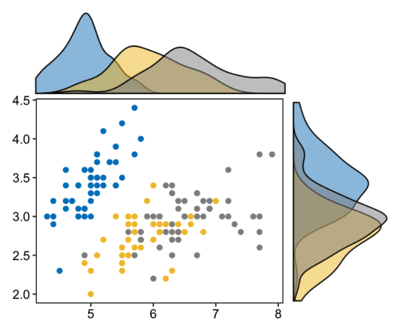
\includegraphics[width=2in]{fig/dist.png}
 \end{center}
 \caption{Probability distributions from $x$ times $y$.}\label{joint}
\end{wrapfigure}  Imagine, in Figure~\ref{joint}, that  we
discretize the horizontal and vertical features into ten equal-width bins.
Once discretized in this manner,   then  this data
has \mbox{$(S=10)^{N=2}=100$} states. But since the distribution of these features are skewed (particularly, the horizontal blue values), many of those  
states occur at zero frequency
(evidence: see   the white space in
Figure~\ref{joint}). 

This {\em Druzdel effect}
(that most of the potential states within the software are never visited)
has been observed in practice.
%many times
%(see Table~\ref{evidence}).
For example, Druzdel's~\cite{druzdzel2013properties} 
logged the frequency of observed states in  
a medical diagnostic system that monitored anesthesia patients in intensive care. 
Of the 525,312 observed states, one state occurred over half the time;
49 states covered 91\% of the probabilities; and the remaining states occurred vanishingly rarely
(at frequencies ranging from $10^{-6}$ to $10^{-22}$).
Similar effects (where most  states  
are rarely visited) has been reported many times, albeit by different names.
Stallings~\cite{stallings09} comments that operating systems often assume
{\em  locality of  reference};
 i.e. that  program
 execution does not dash across  all the code
 all the time but instead is mostly
 focused  on a small part of
 the memory or instruction space.
 Lumpe et al.~\cite{lumpe2012learning} report  studies tracking decades of  work in dozens  of  open-source projects. In  that code base,
 most classes are written once, revised never. Also, most  of  the  defect-inducing
 activity is centered around a small number of rapidly changing classes. Similar observations (where most activities happen in  small parts  of the code)  have been seen in software from AT\&T~\cite{Ostrand04}, NASA~\cite{Hamill09},
 and in   widely used open-source compiler tools (GCC~\cite{Hamill09}). 
 

One explanation for this Druzdel effect is that when code runs, it only visits the $v$ states 
approved by the combination of its internal logic. This space can be far
smaller than $S^N$ (so $v\ll S^N$). 
Explanations, or controllers, of  software that visits  
\mbox{$v\ll S^N$} states only need to explore $\log_2{v}$ ``key'' features.
For example, Zhang et al. report that by
generating tests only for the main branches in the code, even applications that process large cloud databases can be tested via just a few dozen inputs~\cite{Zhang20}.


 The number of   keys features in a data set can be inferred from
the number
of examples  required to model that data.
$N_i$ features with $S$ states can visit $v_i=S^{N_i}$  states.
Hence, we can say that $v_i$ observed states are controlled by
$\log_S{(N_i)}$ key features. The maximal case (that leads to most key features)
is $S=2$; i.e. everything is binary. 
How many binary features are needed to form these state spaces:
\bi
\item
 Druzdel found  $v_1=49$ commonly reached states.
\item
Yu et al.~\cite{zhe19} report that
security violations in 28,750 Mozilla functions can be successfully modeled via an SVM with \mbox{$v_2=271$} support vectors. 
\item Tu et al.~\cite{tu20} report that defect labeling  in  $6000$ commits from Github
can be successfully modelled via a SVM with \mbox{$v_3=300$} support vectors~\cite{tu20}. 
\ei
Assuming binary keys, then we estimate
that the  systems explored by Druzdel, Yu, Tu, et al.
are   controlled
by at most 
$N_1,N_2,N_3\approx 6,9,9$
key binary features.
The next section argues that such small sets of key features
can be used to simplify many SE applications.

 
\section{  How Can ``Keys'' Help  Requirements Engineering? }
  
 
 \subsection{An Informal Example}\label{keyseg}


Suppose an analyst wants to understand 
the requirements for 
a fuel-efficient lightweight car with good acceleration. The file
{\em auto93} (from the UC Irvine ML
  repository) describes hundreds of  cars and their number of cylinders $c$, horsepower $h$, displacement $d$ (a.k.a. size of car), year of release $y$ and country of origin $o$.
From this data, our analyst could learn   Equation~\ref{model1} using
(e.g.) linear regression:
 
{\small
\begin{equation}\label{model1}
\begin{array}{r@{=}l} 
  \mathit{weight} &
 60.7{\times}c +
      5.2{\times}d +
      4.1{\times}h +
     13.7{\times}y +
    -48{\times}o +
    234.2 \\     
  \mathit{mpg} &
     -0.6{\times}c +
     -0.1{\times}d +
     -0.1h +
      0.6{\times}y +
      1.2{\times}o +
     -12.9 \\   
 \mathit{accel} &
      0.1{\times}c +
      0.1{\times}d +
     -0.1h +
      0.1{\times}y +
     -0.2{\times}o +
     21.2\end{array} \end{equation}
     }
     

While this model certainly summarizes the data, 
Equation~\ref{model1} is not yet statement of what {\em little}
we need  to {\em most improve} 
weight {\em and} mpg 
{\em and} acceleration.
To find that succinct plan, our analyst could run a large number
of what-of queries across a large population of cars.
A standard tool for this purpose is a   genetic algorithm that 
(a)~mutates population of cars,   (b)~scores the mutants
on the above three equations, then (c)~selects the best scoring mutants as parents for
the next generation of mutants.
That genetic algorithm approach may not scale to large problems.
Peng et al.~\cite{kewen21} has applied genetic algorithms to explore $C=10^4$ software configuration options
(in order to optimize for $G=2$ goals). In that application,
the $O(GC^3)$ non-dominating sort procedure of the NSGA-II~\cite{deb02} genetic algorithm took hours to terminate.  

A (much) faster approach, that generates succinct statements from the data, uses the keys effect, as follows.
The following KEYS0 algorithm assumes that there exists a small number of feature ranges that occur with different frequencies in desired and undesired outcomes. These can be identified via a little random sampling combined with the pruning of unpromising regions. That algorithm works as follows:
\be
\item   {\em Cluster.} Select a few random points to find two
distant points $P_1, P_2$  within the data. Sort them such that point $P_1$ is better than $P_2$
(if exploring multiple goals, use some domination predicate to rank the two items).
Mark the data   {\em best, rest} depending on whether it is
closest to  
$P_1,P_2$. Readers of the AI literature will recognize this as the FASTMAP
clustering algorithm~\cite{faloutsos1995fastmap}.
\item  {\em Contrast:} Look for
feature ranges
with very different frequencies in {\em} best
and {\em  rest}. 
Divide numeric features into 
$\sqrt{n}$  sized ranges. Combine adjacent ranges that have similar {\em best, rest}
frequencies. Rank feature ranges, favoring those that are more frequent in {\em best} than {\em rest}. Print the top-ranked range. 
\item  {\em Prune and recurse.} Discard anything  that does not match the top  range.
Loop back  to step1.
\ee
 When executed on   {\em auto93},
KEYS0
terminates in two loops after evaluating  four cars.
It makes two recommendations:
  ``cylinders $\le$ 4''
and ``origin==3''. 
Figure~\ref{auto} marks with an arrow the position of the data
selected by KEYS0.  In a result consistent with the presence of keys 
{\em auto93}, we see that by examining just four\begin{wrapfigure}{r}{2in}
\vspace{-5mm}
    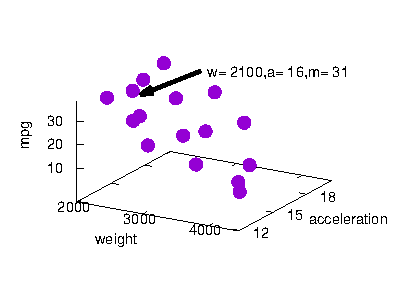
\includegraphics[width=2in]{fig/introduction.eps}
    \caption{16 clusters of 398 examples from  {\em auto93}. Arrow
    shows  region found by KEYS0.}\label{auto}
\end{wrapfigure}
examples and asking about two
ranges, we   found a useful
region in the data. Further improvements are
possible, of course (e.g. the  acceleration is still
mid-range in the final selected data). Nevertheless,  
 three  aspects of this example that are worthy of
careful attention. 

Firstly, as far as we can tell, the model learned by KEYS0 is not apparent
within the output of standard learners
such as Equation~\ref{model1}. That is, keys-based reasoning can find
structures invisible to other learners.

Secondly,  as  bragged in the introduction,
this example shows that keys can reduce   modeling effort
by two orders of magnitude. Recall  that KEYS0
found the region marked with an error in 
Figure~\ref{auto} using labels from
only $4/398\approx 1\%$ of the cars
in {\em auto93}. This reduction in the labeling effort was achieved
using a method taken from  semi-supervised learning~\cite{van2020survey}
(specifically: rather than labelling all  data,
KEYS0 first found clusters of similar  cars, then  only asked   one label per cluster).



Thirdly,  while KEYS0 is a useful tutorial
 introduction to keys-based reasoning,
  this code
 is a hastily-written throw-away prototype with obvious shortcomings
 and room for improvement.  Later in this proposal, we will discuss methods to
 address those shortcomings and make those improvements. 


\subsection{A Formal Analysis}
This section argues that the informal
example shown above (about cars)
is representative of a much more
general process; i.e. requirements engineering (RE). 
Specifically, requirements engineering  means navigating a space of choices
so if the keys effect can reduce that space of choices, then that
would lead to faster RE.

 Traditional  requirements
engineering was an activity
that happened at the start of a project. But in the age of
continuous deployment,  at any time in the project, developers will stop to reflect on what to do next 
(e.g. every time an agile team reflects what part of the backlog they need
to explore next).  Hence, in Table~1, we say that as  PI Menzies and Zimmermann~\cite{timzim13}
explore the space of possible queries,
  they are doing requirements engineering for software analytics. Also,
  when Briand~\cite{Abdessalem18} applies decision tree learners and neural nets to cyber-physical systems,
  we are learning the requirements for how to certify those systems. Finally,
  as PI Menzies, Hu, Tu et al.~\cite{zhe19,tu20} using active learning to seek vulnerabilities
  in source code files, they
  are doing security requirements engineering. 

 
As to the  space searched by requirements engineering, Zave and Jackson~\cite{Zave97}   characterized RE as
the application of  knowledge  $K$ to a   specification $S$   to achieve 
requirements $R$; i.e.
\begin{equation}\label{one}
K \wedge S \vdash R\end{equation}

Jureta and Mylopoulos et al.~\cite{Jureta08} take issue with
 Equation~\ref{one} 
 saying that it does not allow for partial fulfillment of
requirements. Hence, Zave and Jackson's formalism    leaves no room for one 
partial RE
solution to be {\em better} than another.
Another drawback with Equation~\ref{one} is those   preference criteria
 (or, ``nice to have''
requirements) are left out of the framework, with no substitutes to compensate for this omission.
Jureta, and Mylopoulos et al. preferred alternative to Equation~\ref{one} is
\begin{equation}\label{two}K*,P* \skepcon G*,Q*,A*\end{equation}
where
$\skepcon$ is a nonmonotonic  entailment operator
   (so we can change our mind) and
$A$ are  preference criteria which  Jureta, and Mylopoulos et al.
call ``attitudes'' (.e. some   general evaluative
reaction such as ``I like Y'' or ``I like Y more than Z'').
Also, in Equation~\ref{two},
Jureta, and Mylopoulos et al. replace 
the specification $S$ with  a set of relevant
plans $P$ that could possibly be applied.
Further, they switch the hard-and-fast requirements $R$ with 
constraints $Q$ and  goals $G$. Another nuance is that Jureta, and Mylopoulos et al.
use  
$A*,P*,Q*,G*,K*$ to denote the union of  compulsory
and optional parts of $A,P,Q,G,K$. 


 \begin{figure*}[!b]
%\begin{mdframed}
 
   ~~~~~ 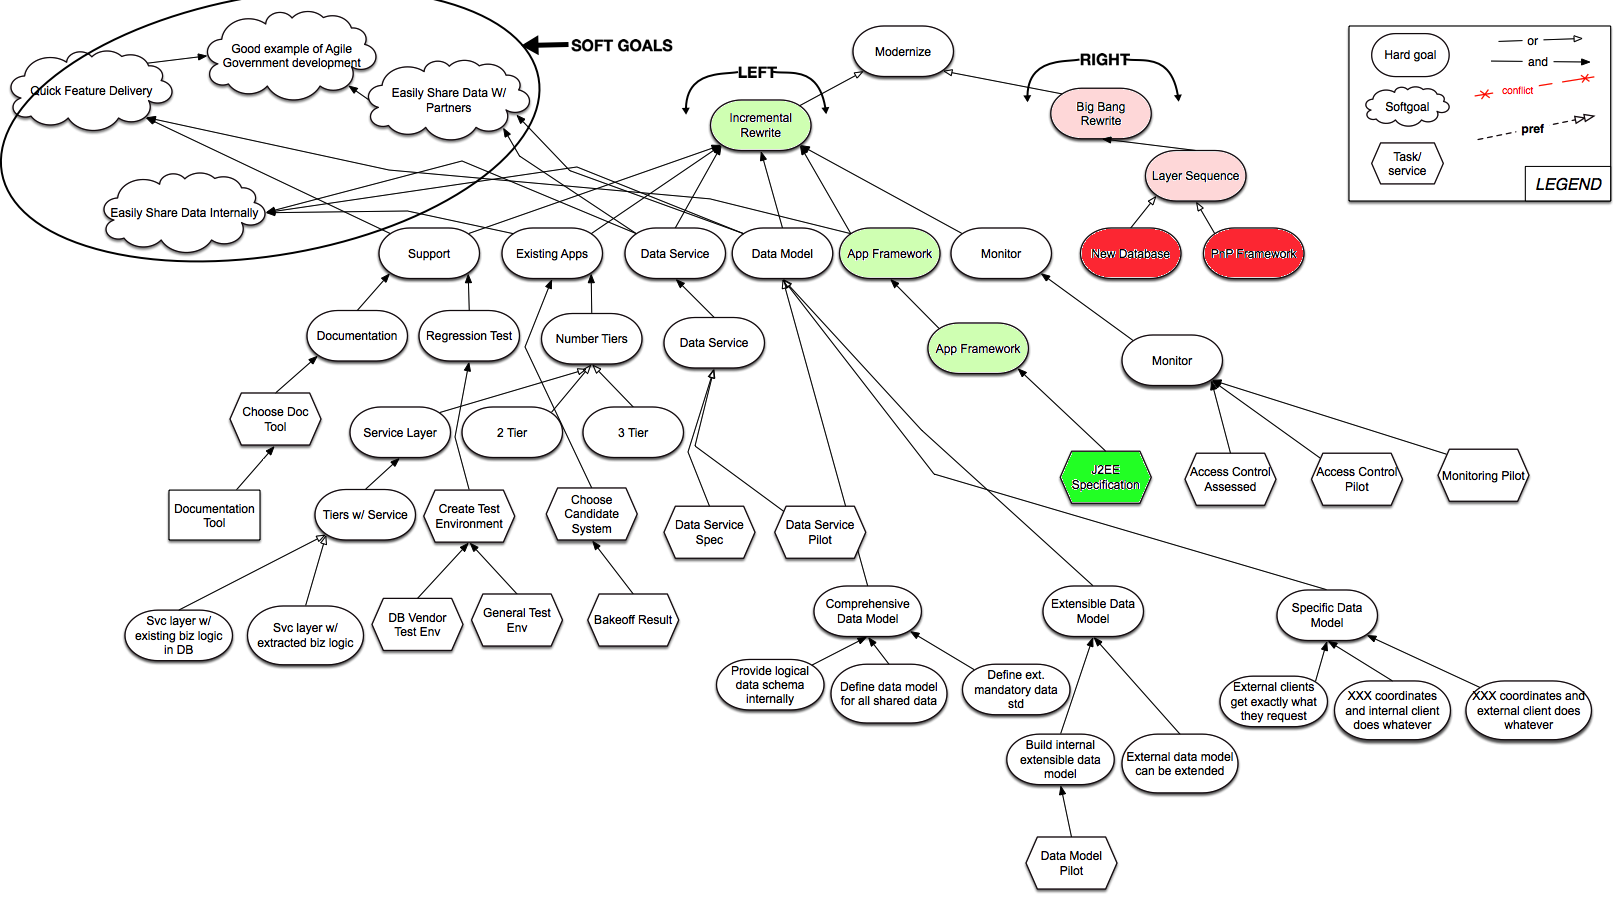
\includegraphics[width=6in]{fig/AOWS_modified}
 

%\end{mdframed}
\caption{A requirements model for
   IT System modernization.    The three keys
of this model are the leaf nodes shown in red and green (see text for an explanation of why these are 
the keys). }
    \label{fig:aows}
\end{figure*}For example,  
  \fig{aows} shows a  requirements model about IT System modernization tasks such as 
the Y2K problem (moving from 2 digit to 4 digit years);  reacting to vendor decisions to end-of-life operating systems and database products; and
 improving architectural support for new capabilities (e.g.,
 support
for mobile devices).
The model in \fig{aows} comments on the refactoring, re-architecting, and  redesign  of
existing  systems. 
Note that the model has dozens of decisions and   a few top-level goals shown circled top right: ``Good Example ...'', ``Easily Share Data Internally'', ``Modernize''.   
In that diagram,  $G*$ comprises the compulsory
topmost node (``modernize'') as well as optional ``soft'' goals shown top-left. 
There are no conflicting
goals so $Q*=\emptyset$. In the domain, the  preference attributes $A*$ is to find the least coast solution
that covers all the compulsory goals and as many soft goals
as possible. That said, for the purposes of this example we assume that cost of all the decisions is \$1 (which we could update if domain knowledge $K*$ includes that information).
Most importantly, the diagram has 24 leaf nodes so the size of $P*$ is $2^{24}$.  In our
experience, business users take a long time to debate that space of options.



\begin{wrapfigure}{r}{3in}
    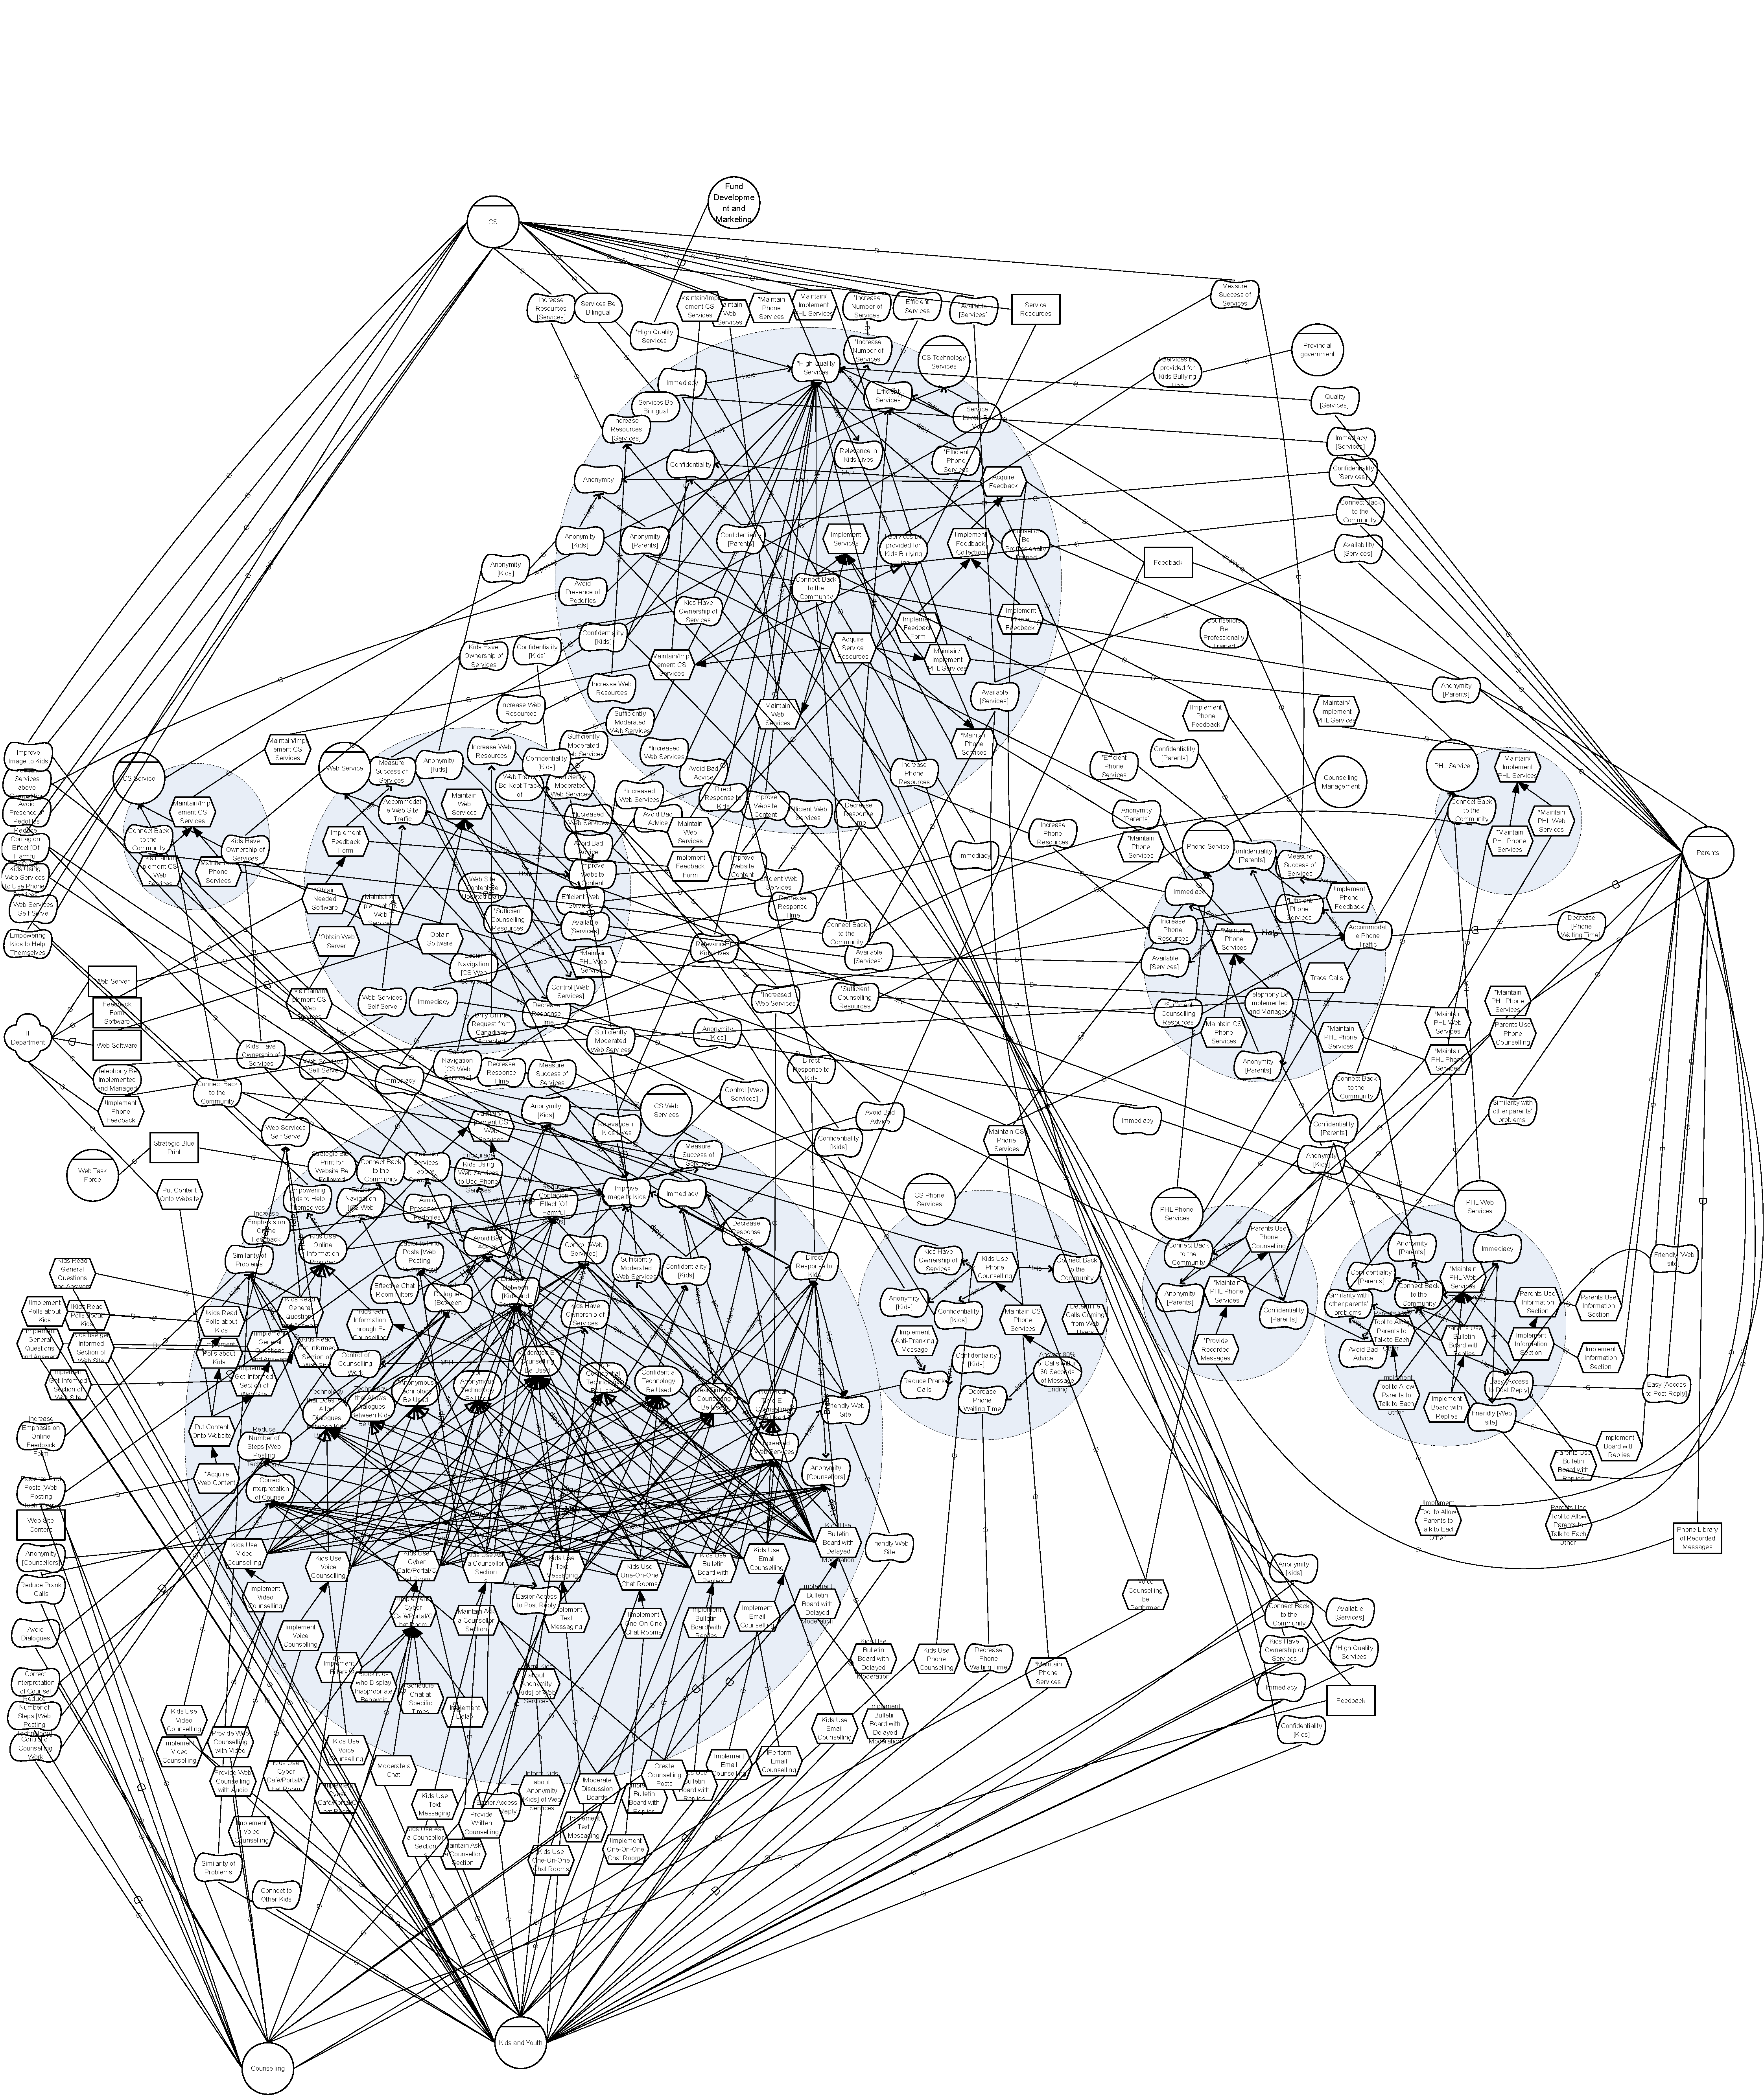
\includegraphics[width=3in]{fig/CSServices.pdf}
    \caption{Options for services in a CS department. 351 nodes and 510 edges.  }\label{fig:auto}
\end{wrapfigure} The keys
are the subset of $P*$ that have most effect on the system.
In  \fig{aows}, those keys are 
the two red and one green decisions in \fig{aows}. To see this, note that
the right-hand side of the model has no connection to the top goals. Hence,  two sensible
  decisions for this model would be to deny the leaves marked in dark red, thus disabling the right tree.
 As to the left-hand side of the model, the leaf marked in dark green (``J2EE specification'') selects
  the shortest left-hand-side sub-branch with the fewest leaves. If the goal is to achieve the most high-level goals
  (at least cost), then it is also sensible to take this single dark green leaf. Why? Well,   making any other decision
  on the  left-hand side of the model  will significantly add to the overall cost of the solution, since all those other decisions
  require many more conjunctions of decisions\footnote{It is reasonable to ask what to do if users reject this analysis  and  explore the deeper branches on the left-hand side.
  This would tell a requirements engineer that ``minimizing cost" is an optional part of the attitudes $A*$ which 
   would lead to new alternatives.}.
 

 In \fig{aows}, the keys are simple to detect via a visual inspection (just look for the shortest subtrees). For more complex models, such visual inspections are not so informative.  
\fig{auto} shows a requirement engineering of the Toronto University Department of
Computer science (written by Steve Easterbrook and Jennifer Horkoff~\cite{mathew2017shorter}). Not only 
is the model hard to visualize, like many requirements models, it can generate
contradictory  conclusions (since different stakeholders want different goals).
Inference engines that explore  models containing contradictions
must struggle to find the largest subset of the knowledge that does not connect incompatible conclusions. 

\begin{wraptable}{r}{1.9in} 
    {\small\begin{equation}\label{suba}
     \begin{array}{r@{~}c@{~}l}
       K &\subseteq& \mathit{domain\; knowledge} \\
       M &\subseteq& \mathit{maybes}\\    
       G &\subseteq& \mathit{goals}\\
       K \wedge M&  \vdash & G\\
       K \wedge M & \not\vdash& \bot
       \end{array}
      \end{equation}} 
\end{wraptable}
In the AI community, exploring models looking for maximal consistent
subsets is called {\em abduction}. Poole~\cite{Poole1994} describes abduction
 as follows.
 When we reason about knowledge  $K$, we make {\em assumptions}
     (denoted $M$ for ``maybe'')
     about either (a)~initial
     facts or (b)~how to resolve contradictory decisions.
     In Poole's framework, there is no separation of  compulsory and optional components:  
     things are either achievable or not and  inference engines must strive
     to achieve as much as possible.
     As shown in Equation~\ref{suba},
     in the general case, only some subset of the theory can
     be used to achieve some of the goals $G$ using some subset of the maybes,
     while avoiding  contradictions (denoted $\bot$, computed from 
     what Jureta and Mylopoulous.
     A {\em world of belief} is a solution that
     satisfies Equation~\ref{suba} and which is not a subset of some other world.
       In the general case, Equation~\ref{suba} can generate multiple
     worlds $W_1, W_2, W_3...$, at which point we need 
     Jureta, and Mylopoulos et al.'s preference knowledge
     (the attitudes $A$) that can tell us which model is preferred. For example,
     for \fig{auto}, the attitude was to achieve as many goals as possible,
     at least cost.
     Within a world,   some maybes $M_j$ can depend on other maybes $M_i$;
     i.e. $M_i \vdash M_j$. The top-most maybes $M_0$
     (that depend on nothing else) are what   Jureta and Mylopoulous would call
     the $P*$ since they tell us how to achieve
     different outcomes (i.e. how to build different worlds).
 
 

Bylander et al. 
 warns that this abductive search is NP-hard~\cite{Bylander1991}.
 It is easy to see why.
When exploring all the subsets in Equation~\ref{suba},
 we should expect
very slow runtimes. Bylander et al.'s pessimism
 has confirmed empirically by PI Menzies et al.~\cite{menzies1996applications}, theoretically by Abdelbar et al.~\cite{Abdelbar:2004},
and then again empirically by
Ernst et al.~\cite{ernst12caise}.

The experience to date is that methods that efficiently explore medium to large
RE models like \  \fig{auto} require
restrictive assumptions on nature
of the model. For example, at RE'17, PI Menzies presented an algorithm called SHORTER which could  compute Equation~\ref{suba}
for RE models with hundreds of nodes in a matter of minutes (while other approaches, such as NSGA-II~\cite{deb00a} took over an hour to terminate~\cite{mathew2017shorter}).
But that SHORTER method made restrictive assumptions about  (a)~the allowed ranges of values, (b)~the nature of the edge constraints, and (c)~the overall shape of the model.
Hence, SHORTER cannot be recommended as a general approach to faster requirements engineering.


That said, even though SHORTER  failed to provide a general approach,
it did suggest how such a general approach might be achieved. 
The SHORTER paper did   confirm the presence of keys within half a dozen
RE models, including \fig{aows} and \fig{auto}\footnote{
Specifically   decisions on less than 12\%  of the features
was enough to minimize cost and maximize goal coverage.}.
The salient point  to be made here is  
SHORTER  did  not use keys to reduce
the search space {\em even though those models contained keys}.

Hence, for the rest of this proposal,
{\IT} will try placing the cart before the horse. Instead of running
slow inference engines that report keys in the output,
{\IT} will be based on algorithms (like KEYS0) that assume keys, then use that assumption
to restrict the search space.  


\section{ Technical Details}
\noindent
Before turning to research questions, we need some lower-level details:
\bi
\item \S\ref{desire} lists  desired properties of faster anytime requirements engineering;
\item \S\ref{aa} lists  various methods for building systems with those properties;
\item \S\ref{howtest} discusses how to comparatively evaluate those alternatives.
\ei

\subsection{Desired Properties}\label{desire}

Human-in-the-loop anytime tools like {\IT}
 must take care not to
 overload their human partners with too much information. 
 One way to reduce cognitive overload
 is   the {\em contrast trick} used in KEYS0 i.e. the differences between two similar
 concepts are much smaller than a full description of every detail of
 those concepts~\cite{borges2012learning,kelly1969clinical}. Hence, when showing a human 
 hierarchically clustering data, a contrast
 set that distinguishes sibling clusters may need only one or two features.
  
Another important requirement for {\IT} is repeatability.
Recent statements about ethical AI from the
Microsoft, IEEE, and the European Union~\cite{EU, MicrosoftEthics, IEEEethics} stress the need for
{\em accountable} AI. Ideally, some third party can reply to old design decisions and when they disagree, they can perform a ``what-if''
query to determine the impact of changing that decision.
Note that keys are very important for simplifying  accountability.
Evidence: recall
from the end of \S\ref{aboutkeys} that seemingly complex systems were controlled
by just a handful of keys. For systems like that: (a)~the number of
key decisions required to control that system will be very small; and
(b)~the effort required to explore alterations to those keys will also be manageable.

 Since our aim  to increase human insight
 about a domain, it is unlikely that neural approaches
 (with their opaque models) are suitable for {\IT}.
That said, we take inspiration from research into
methods that try to  generate
explanation   neural networks. The LIME algorithm for neural nets~\cite{AIFLIME}
has been   successfully applied to 
a wide range of algorithms (not just neural nets
but also   random forests, naive Bayes)
since it is ``model-agnostic''; i.e. it makes no
assumptions about the model generating the data.
For example, when working with SE data,
Lowry~\cite{lowry98} comments that each ``if'' statement divides
the state space into different regions, each of which
might have dramatically different properties.
Hence we should not assume that the 
underlying model is smooth and differentiable
across the whole space. Therefore, it is unlikely we can use
(e.g.) numeric optimizers like SIMPLEX~\cite{nelder1965simplex} or 
(e.g.) gradient
descent methods that assume that data generator
is some parametric form that follows some
partial derivative in the data. What seems more likely is that all the different effects in SE data have to be isolated in different clusters (as done in KEYS0).




\begin{wraptable}{r}{2.3in}
{\small
\begin{array}{rcl}
\textit{worse}(x,y)& =& \textit{loss}(x,y) > \textit{loss}(y,x)\\
\textit{loss}(x,y)& = &\sum_j^n -e^{\Delta(j,x,y,n)}/n\\
\Delta(j,x,y,n) & = & w_j(o_{j,x}  - o_{j,y})/n
\end{array}}
\caption{
Zilter's indicator, from~\cite{Zitzler2004IndicatorBasedSI}. $y$ defeats  $x$ if $x$ ``losses'' most. Here, 
 ``$n$'' is the number of objectives
 and  $w_j\in \{-1,1\}$   if want to
minimize/maximize goal $x_j$ (respectively).}\label{zitler}
\end{wraptable}
~{\IT} needs to
supports multi-objective problems where there are multiple,
possibly competing, dependent variables.
Mylopoulos and Chung~\cite{chung2012non}  have written much on
 (a)~software projects have stakeholders and (b)~these stakeholders may have different goals.
 One useful
 way to handle such multiple goals is to express them as different regions
 within a multi-dimensional goal space (one dimension per goal).
 For example, 
 RE researchers like Letier~\cite{heaven2011simulating}    presenting the output of inference output as a cluster within a multi-goal space (otherwise known as ``trade space''). For that reason,
 KEYS0 used a multi-goal ``domination predicate'' to sort the cluster data into best and rest.
 The standard ``Boolean dominance'' predicates says that one example
                                 $x_1$ dominates 
                                another   $x_2$,
                                if $x_1$ is   better than $x_2$ in at least one objective and if $x_1$ is no worse than $x_2$ in all other objectives.
                              KEYS0 used
                              instead
                              the   ``Zitler indicator'' continuous
                              domination predicate ~\cite{Zitzler2004IndicatorBasedSI} of Table~\ref{zitler}.  At ICSE'13 we showed that the number of goals
increased, the Zitler indicator out-performed boolean domination~\cite{sayyad2013value}.


SE models contains often numeric and
symbolic information.
This is particularly true in
safety-critical domains where the model code
contains conditionals that implement
clauses from  legal regulations. 
According, when clustering, {\IT}  needs  
heterogeneous distance measures that can handle both symbols and numbers.  For example, the Aha's distance measure~\cite{aha91} used in KEYS0
(a)~normalizes all numerics zero to
one (min to max), then (b)~declares
that the distance between two symbols is zero if they
are identical (otherwise, that distance is one). Note that once data clustered recursively on the independent variables, 
 {\IT} can support   regression and classification
problems by summarizing the leaves  using 
{\em mean} or {\em median},
(for regression problems) or 
{\em mode} (for classification problems).

Once data is clustered, then it can support active learning~\cite{settles2009active}.
Machine learning algorithms can achieve
better performance with fewer labeled training examples if the algorithm is active in selecting
the training data from which it learns. For example, recall that the KEYS0
example from \S\ref{keyseg} only needed to look at the 
dependent feature labels of four cars
(our of 398) to achieve its results. To do this, KEYS0 first
made extensive use of clustering and contrasts within
the independent features {\em before} it accessed the labels
on the dependent features. 
Active learning is important for {\IT}   since
repeated studies show that labeling SE examples (i.e. setting
the dependent variables) can be expensive and error-prone process~\cite{yu2020identifying,tu20}. Hence it is vital in SE applications
to reduce the number of labeled examples used during training. 
 
 \subsection{ Alternate Approaches}\label{aa}
 Having described the desired properties of {\IT},
 we note that some of these properties exist
 in rival approaches:  
sequential Model Optimization (SMO)
and interactive Search-Based 
SE (iSBSE). 
This section describes iSBSE and SMO.

 Sequential Model Optimization (SMO) are   active learners
that reflects on the evidence seen to date  select the best
example to label next~\cite{JMLR:v17:15-047,nair18tse}:
\bi
\item
Given a small initial sample, SMO learns
a model that  can report
not just mean predictions, but also a measure of variability around that mean. 
For example, when SMO  learns
Gaussian Process models (GPM), the usual  acquisition function
 probes the model looking for (e.g.) regions with best mean predictions and highest
variability.
SMO is used in domains where decisions have to made as soon as possible,
having made the fewest  observations possible about the domain.
For example, Golovin~\cite{10.1145/3097983.3098043} reports  Google's
use of SMO for runtime reconfiguration of Google
cloud services.
\item
Previously we have explored SMO for configuring software devices~\cite{JMLR:v17:15-047}.
We found that that standard SMO methods  like
GPMs do not scale well for software systems with more than a dozen variables~\cite{10.5555/3013558.3013569}. For example, in SE, the state-of-the-art in this
area using GPMs for optimization was limited to models
with around ten decisions~\cite{10.5555/3013558.3013569}.
Other approaches to SMO do better than GPM. For example, Begrsta' TPE algorithm~\cite{bergstra2011algorithms}
uses a Naive Bayes
classifier to model old data divided into ``top'' and ''bottom''. New candidates
are then assessed by their likelihood of belonging/avoiding top/bottom (respectively).
\ei
As to search-based SE~\cite{harman2012search}, these
are algorithms that explore
SE problems to   trade-off between multiple completing goals:
\bi
\item
Modern SBSE algorithms do not generate single solutions
but rather return an envelope    of preferred solutions spread across a
{\em Pareto
frontier} of solutions
scored via
  different objectives.
By clustering and browsing the Pareto frontier, requirements engineers  can explore different ways to
find the {\em least} cost mitigations that enable {\em  most} requirements.  Unlike
traditional optimization methods (e.g. SIMPLEX~\cite{nelder1965simplex}),
search-based SE makes no assumption that
all goals are achievable. Instead,
search-based SE makes the more realistic
assumption that to win on some goals might mean
trading off on other goals.
Classic SBSE algorithms include evolutionary
algorithms like simulated annealing~\cite{rothman1942automatic} or genetic algorithms~\cite{holland1992genetic}
and differential evolution~\cite{Storn1997}.
More recently, much work has explored better ways to select better individuals (e.g. NSGA-II~\cite{deb2002fast}) or how to decompose all the solutions into useful subsets (e.g. MOEA/D~\cite{Zhang07}).  \item
Standard SBSE is ``black-box''; i.e. these algorithms run and produce results,
even if users have no understanding or input into how those results are obtained.
Interactive SBSE~\cite{amal2014use,araujo2017architecture,mkaouer2016interactive,lin2016interactive,marculescu2013objective,simons2014interactive,palma2011using,tonella2013interactive,ramirez2018systematic,goyal2018identifying,do2016incorporating} is a variant of SBSE that tries to include humans     in the reasoning process. More specifically, given a range of options,
iSBSE tries to find which preferences are most important to users. iSBSE methods wrap some underlying inference engine
in an addition ``what-if'' that is  used to rank potential questions {\em before} they are
passed to a user.  
For example, 
Palma et al.~\cite{palma2011using} wrap a  state-of-the-art constraint solver
(the MAX-SMT algorithm~\cite{kautz96}). 
Other approaches are machine learning to summarize numerous
what-if queries~\cite{araujo2017architecture}. The model learned in this way can be used to
determine what questions most affect the optimization
outcome. Yet other approaches let users reach in
and directly alter the preferences on the underlying
search-based model (e.g. see the swarm intelligence method of Ferreira et al.~\cite{do2016incorporating}).
In a few limited domains, we have seen that {\IT}-like methods
run faster and produce smaller models than SBSE~\cite{DBLP:conf/re/FeatherM02} and iSBSE~\cite{lustosa21}. But, prior to this research proposal,
we are unaware of any  serious study that checks
the general effectiveness of
how much data mining
methods like {\IT} compare to evolutionary iSBSE and SBSE methods.
\ei
We propose SMO and iSBSE as rival technologies to {\IT} since they
their algorithms share some of the desired properties of {\IT}
described in \S\ref{desire}.
For example,  like KEYS0, SMO strives to make as make effective conclusions uses the fewest labels. For another example, like KEYS0, iSBSE tries
to reduce the amount of work a user must perform in order to control an inference device.
 But while SMO and iSBSE have some overlap with KEYS0 (and, more generally, with {\IT}),
 our preliminary results suggest that:
 \be
 \item
 {\IT}'s data mining approach can find solutions
 much faster than SBSE and iSBSE.
 \item 
 {\IT}'s data mining approach scales better than SMO and leads to fewer questions
 to the user.
 \ee
 We stress that these two points are preliminary results and more research (to be conducted as part of
 this proposal) is required.
 

\subsection{Evaluation Methods}\label{howtest}
% In this section, we pose the following research questions.
% \begin{changemargin}{0.6cm}{0cm} 
%  \bi 
% \item[RQ1:] {\em How should {\IT} uncover the keys?  } 
% \item[RQ2:] {\em How to detect when {\IT}'s keys-based reasoning might not work?}
% For this question, we need a detector
% that can report when tools like {\IT} will be useful
% or useless.
% \item[RQ3:] {\em Across many data sets, how prevalent are keys? }
% Just how widespread is the keys effect?
% What happens when   the keys detector (from RQ2)
% is applied to much of the SE data used in the software
% analytics? 
% \item[RQ4:] {\em Where do keys come from?} If the results of RQ3 shows that keys
% are highly prevalent,   then we must ask a basic
% question: where do keys come from?
% \item[RQ5:] {\em How to reason with keys and {\IT} in the face of   human error (or indecision)?}
% Most of the past results that
% found
% keys assumed that when humans and AI ask each other
% questions, then they will receive correct answers. But humans make mistakes
% and teams of humans may not even agree on what ``correct'' means. 
% So, how can {\IT} cope with that?
% \item[RQ6:] {\em What are the limits to  this use of {\IT} and keys?  }
%  Current results suggest that applications like
% the vision system of autonomous cars need complex  deep
% learner to handle (e.g.) 10,000 wavelets coming from the signal processing system~\cite{zhu2017deep}.
% But how complex does data
% need to be before simple methods like keys fail and complex methods like
% deep learning becomes essential? 
%  \ei 
%  \end{changemargin} 

\begin{wrapfigure}{r}{2in}
 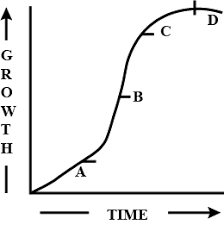
\includegraphics[width=2in]{fig/growth.png}
 \caption{Model Building. (1) initial work; (2) some progress; (3) diminishing returns; (4) performance plateaus; (5) normal operation; (6) some problem; (7)  fixed;  (8)   collapse, after which the  cycle might start again.  }\label{intoai}
\end{wrapfigure} The case studies for this research were discussed above, in 
Table~\ref{casestudies}.
Using that case study material,
 this research will
 use the  incremental model   framework of 
PI Menzies, Hu,Tu et al.~\cite{zhe19,tu20} to evaluate
keys versus iSBSE versus SMO.
This framework is shown in Figure~\ref{intoai}.  
Here,  AI and humans team up to solve problems. Whenever humans make a decision
about a certain example (i.e. they supply a label saying that an example  is ``desired'' or ``undesired''),
then the decision count on the  $y$ axis is incremented.
At that point, the AI uses the examples labeled so far to
build some model.
That model is then scored  using real-world data
and that  score becomes
a new point on the $z$ axis. 

Note that, in Figure~\ref{intoai},
 one method for building models (e.g. keys or iSBSE or SMO)
 is better than another if  it leads to
higher {\em z = goals} are achieved with fewer $y=decisions$.  

 Other measures of interest from Figure~\ref{intoai} 
are (a)~how long before  models   need
repair (see the segments labelled ``5'' and ``6'' in Figure~\ref{intoai}) and
(b)~how much effort is required for that repair (see   segment  ``7''); (c)~how much human time (measured in seconds)
is required for interacting with the AIs; and (d)~how much CPU
time is required to update the models.
With these measures, we can compare the results
from {\IT}, iSBSE, SMO to check
if {\IT} is better for generating  
(with less effort) simpler models with superior performance (as measured by some domain-specific criteria).


                
~{\bf OTHER EVALUATION DETAILS:}
Since we have many treatments (variations of keys-based reasoning, iSBSE, SMO)
and since   our algorithms may be  stochastic in nature\footnote{For
example, the genetic algorithms used in iSBSE often employ random mutation.}, we will have to run the rig of Figure~\ref{intoai}, many times, using different random
number seeds. The different treatments will then be compared
with non-parametric effect size and significance tests
(e.g. A12~\cite{Arcuri} or Cliffs~\cite{hess2004robust}, and bootstrap~\cite{EfroTibs93}).

Our studies will divide into two. {\em Automated studies} will make the decision on the y-axis
of  Figure~\ref{intoai} using historical data in order to assess different variants
(of keys, iBSE, SMO).
Once those automated studies cull  the space of potentially useful variants, then we will switch to {\em human-in-the-loop
studies} where humans are making the y-axis decisions of Figure~\ref{intoai}.
We anticipate running 100,000s of automated studies and 100s
of human-in-the-loop studies.

 For the human-in-the-loop studies, we will take advantage
of the Mechanical Turk crowd-sourcing platform.
   Mechanical Turk   connects workers (i.e., the people performing the tasks) with requesters (i.e., the people creating the tasks)~\cite{mturk}.  This platform has been used extensively in software engineering applications~\cite{mao15} and for the evaluation of software engineering research (e.g., \cite{Stolee:2010:EUC:1852786.1852832,stoleeesem2013,Fry:2010:HSF:1912607.1913292}). 
   
When we discussing the use of Mechanical Turk,
colleagues often ask ``for the SE
requirements models you want to build, can you find enough SE subject matter experts
within the Mechanical Turk population?''. In reply, we say that have had much recent success with such crowd-sourced studies that require crowd workers with SE competence~\cite{wangicse19,8813275,wang2020isense2}\footnote{Including
one distinguished paper, awarded at ICSE'19~\cite{wangicse19}.}
in the SE tasks described in Table~\ref{casestudies}.
The reason this is possible is that many SE researchers have reported that, with appropriate
controls, it is possible to find such
SE skills in crowd workers
(e.g. see Stolee and Elbaum at  ESEM
10~\cite{Stolee:2010:EUC:1852786.1852832}, and
Wang et al.  ICSE'19~\cite{wangicse19}
and Fry and Weimer at 
ICSME'10~\cite{Fry:2010:HSF:1912607.1913292}).
Those controls include 
{\em pre-screening} that that   quickly select
relevant workers; and {\em ``gold'' standard tasks}
where the answer is known and workers are disqualified if
they fail to answer the gold questions correctly. In practice,
pre-screening and gold questions prune 30 to 60\% of the participants,
leaving behind enough workers
with enough SE skills to explore the case studies
of Table~\ref{casestudies}.

                 



\section{Research Questions}

\noindent The introduction of this proposal offered two goals:
\bi
\item
{\em Goal1:}
is to test if the  keys-based {\IT} approach enables faster anytime requirements engineering that reduced CPU and human effort to build
models by a factor of 10 to 100. 
\item
{\em Goal2:} Develop detectors for the keys effect since this will tell us when {\IT} should not be used
\ei
In the following:
\bi
\item
Goal1 is addressed by RQ1 and RQ2.  
\item
Goal2 is addressed by RQ3, RQ4, RQ5, and  (to some extend) RQ6.
\ei 
 \subsection{RQ1: How should {\IT} uncover the keys?}
This section discusses methods to
 build a better version of the KEYS0 algorithm of \S\ref{keyseg}.
 
 
 The KEYS0 algorithm of \S\ref{keyseg}
 was a {\em greedy search} in that it prunes half the data at each level of its recursive search.  
 Recently we have begun exploring more global analysis where the whole
 cluster tree is generated, after which time the algorithm hunts around all nodes looking for features to prune
 and features to keep. Greedy algorithms run faster but global algorithms use more information about the data.
 Which works best? Or is there some way to amalgamate the two approaches (e.g. some local search in the style
 of MaxWalkSat~\cite{kautz96})?
 
Also, KEYS0 cluster the data via hierarchical random projections. There are so many other ways to cluster data\footnote{https://scikit-learn.org/stable/modules/clustering.html} that it would be useful to explore other methods.
For example, if the data is particularly complex, is there any role for other algorithms such as 
 a neural autoencoder?  More generally,
 can we refactor the current KEYS0 algorithm into some object-oriented
 design with abstract super-classes like ``cluster''
and concrete sub-classes for
 different (e.g.) clustering algorithms? Such a refactoring
 would turn the above code into a workbench within
 which multiple algorithms could be mixed and matched
 in an effort to find better explanation algorithms.
 
 
No matter how the clusters are generated, reports must be made to the user
about the difference between the clusters (this difference was reported in \S\ref{keyseg} as the constraints 
 ``cylinders $\le$ 4'' and ``origin=='3'). KEYS0 uses a  simple greedy frequency-based method
 (combine adjacent ranges that have similar {\em best, rest}
frequencies; tank feature ranges, favoring those that are more frequent in {\em best} than {\em rest}; print the top-ranked range)
and there are so many other feature and range ranking methods to try~\cite{ZHAO2021106652,hall2003benchmarking}.
  
For simple data sets like the {\em auto93} data set explored in \S\ref{keyseg},
only 2 constraints are generated before the algorithm cannot find anything else of interest.
Recently we have been exploring larger data sets (with 128 features)
where the keys finder returns very many constraints. Is there an early stopping rule
that can be applied to find enough useful constraints, but no more?

To evaluate the prototypes built for this research question, we would compare keys-variants
with state-of-the-art iSBSE and SMO implementations using the evaluation methods of \S\ref{howtest}.
  

 
 
 
\subsection{RQ2: How to reason with keys and {\IT} in the face of human error (or indecision)?}

A repeated observation is that humans make   mistakes, perhaps
due to high workloads, or their inherent cognitive biases\footnote{Fans
of human rationality should not read the Wikipedia entry on
``human cognitive biases'' that lists 200 ways humans systematically
and repeatedly make sub-optimal decisions.}.
  What happens to any interactive model building process
  like \fig{intoai} if humans
  make a wrong decision in the middle of the modeling process?
  How 
  do we detect, and mitigate that mistake?
  For example, to find errors,
  would some unsupervised outlier detection~\cite{Nam15} suffice? And how  do we repair those mistakes
  Yu  et al. have some preliminary ideas on
  that~\cite{zhe19} (run the latest model over all the old
  decision; revisit all old conclusions that are not approved
 by the latest model) and our task here would be
 find cost-effective ways to find the most errors with the least effort.
  
  
  Another cognitive issue is that humans have different world views. Hence,
  reasoning about teams is very different from reasoning about one or two people.
  In the studies
 mentioned above regarding integration with
 human agency,
  Yu, Tu et al. worked mostly with one or two oracles~\cite{zhe19,tu20}. 
  How might their methods scale to teams? Within the space
  of possible explanations, would we need to
  (e.g.) add in some multi-goal reasoning~\cite{harman2001search} so that
  we can appease the most number of competing goals
  as possible? On the other hand, rather than seek
  appeasement, it is better to report
  separate sets of conclusions where each set
  satisfies a different set of goals
  (e.g. see the Pareto clusters
  in Figure~5 of~\cite{veerappa2011understanding})?
  
  To assess the prototypes built for this research question, we need to implement a
  variety of mistake-mitigation methods and apply them equally to keys-based
  variants as well as   state-of-the-art iSBSE and SMO implementations 
  (and all these would be evaluated using the evaluation methods of \S\ref{howtest}).
  
  
 
 
\subsection{RQ3: How to detect when {\IT}'s  keys-based reasoning might work?}

(This research question is a preliminary to RQ4 and RQ5.)

In this research question,  we seek a detector that can peek
at data sets, then report when tools like {\IT} might be useful or useless.
Currently, we can see three ways to build such detectors.

Firstly, we could apply two algorithms to our data (one that uses
keys and one that does not) to see if the keys-based approach does
as well as anything else. While a possible approach, this first approach would be quite
time-consuming (due to the extensive domain modeling required).
 


 Secondly, keys could be detected if,
 after applying feature and instance selection,
  the reduced data space generates models that perform as well
 as using all the data. Another way to say that is that the
 class distributions in the reduced space mimic the original space. For a discussion on this approach, see
 Papakroni, Peters et al.~\cite{peters2015lace2,papakroni2013data}.
 
 Thirdly, it might be possible to
 run some very simple and very fast data miners run over the data. building models using $N$ or $2N$ features.
 If any learner does no better than another but using only half the features,
 then kill the larger learner and start a new learner that uses
 half the features of the smaller learner. Keys would be defective if the final $N$ value is much smaller than the total number of
 features.  For a discussion on this approach, see
 Holte~\cite{Holte93verysimple}.
 
 
   To build the prototypes   for this research question, we would take all the datasets
   explored in RQ1 and RA2, then sort them by how well the keys-based algorithms scored
   (using the assessment methods of \S\ref{howtest}). We would then check if our detector
   scores were correlated to the assessment scores (i.e. we would check if our keys-based
   algorithms are doing worse in data sets with less keys effect).  
  


\subsection{RQ4: across many data sets, how prevalent are keys?}

The following question is core to this research.
Our experience to date, as shown in Table~\ref{keysSE},
is that the keys effect is quite prevalent. Hence, it is worthy of
detailed that study. Nevertheless,
{\IT} will not work unless domain artifacts have a certain structure; i.e. 
a small number of features control the rest. 
Hence, to evaluate the generality of this proposal,
we need to look at many data sets.

Once we    have an automatic method for determining
 if a data set is amenable to keys (e.g. from RQ3), then we need to run that detector on as many data sets as possible in order to learn the extent
 of the keys effect. 
 Given the current interest in software analytics 
 research (see all the data mining-based papers at SANER, MSR, ICSE, ASE, FSE, TSE, TOSEM, IST, JSS, etc), we do not anticipate any shortage of
 case study data for this research question.
 

\subsection{RQ5:  Where do keys come from?}
Another way  to assess the generality of the keys effect would be to understand what causes them. If we knew that,
 then we could apply the methods  of this paper whenever we see  those causative factors. 
 PI Menzies~\cite{Menzies21}  has speculated 
that  keys arise from  {\em naturalness}~\cite{hindle16}
and/or {\em power-law}~\cite{lin15}  effects. Since programs exhibit the same frequency patterns  seen in human language,  then  {\em  naturally} we would  expect that code usually contains a small number of structures,  repeated many times~\cite{hindle16}.  As to {\em power laws}, suppose programmer2  most understands a small region  of the code written by programmer1.
That programmer  would tend to make  most changes around  that region.  If programmer3 does  the  same  for  programmer2's code,  and  programmer4 does the same for programmer3's code then that, over time, that team would  spend most
of
 their time working on a tiny portion of the overall code base~\cite{lin15}.
 In  such natural code that is  subject
 to  those  power laws, finding a controller for any part of the code  would mean that we also have a controller  for  many other  parts of the code (due to  repetition, due to the small
 size of  the  maintained code  base). 
 
 
To test the above conjectures (that keys come from power laws or naturalness) we could (e.g.)
 built defect predictors from projects that evolved from a small single person into large teams. If power laws cause keys,
 then we would predict that algorithms like KEYS0 would be less/more effective earlier/later in that project life cycle (respectively).
 
 
 
\subsection{RQ6:   How to integrate  {\IT}'s keys-based reasoning with more complex methods?}\label{pm}

Perhaps it is a false dichotomy to say that software artifacts
can/cannot use keys-based reasoning. Another approach might be to   mix and match keys-based reasoning with other methods.

% A complete theory of keys-based reasoning should include methods
% for transition from keys-based to non-keys based methods. As
% new data arrives and as models are updated to handle that new
% data, then it is possible that the keys effect
% might disappear within that model.
% In that case, what would be required would be combining keys-based
% reasoning with other approaches.

In exploring this research question,  we take inspiration from Briand's
work on testing cyber-physical  systems~\cite{Abdessalem18}
(discussed above in the middle of Table~\ref{interact}). That work combines neural
and non-neural methods for exploring a very complex space.
For domains generating very complex data, Briand applies neural nets to learn a summary encoding of the total space. That encoding is used
as a new set of features which a symbolic learn (a decision tree) explores to divide the data into regions of interest (e.g. decision tree
branches leading to data with most/least bugs).
A similar two-tiered architecture could be applied to keys-based reasoning. That is, the very complex model
(e.g. a deep learning autoencoder) could serve as a feature generator. Then, within the space of those generated features, a keys-based
algorithm might find the ``low-hanging fruit'' that controls the space.

As to case studies for this part of the research, the obvious choice
would be deep learning and vision systems for autonomous cars. 




  



\section{Schedule} \begin{wraptable}{r}{3.5in}
{\scriptsize \begin{center}\begin{tabular}{r|l|l|l|}
\cline{2-4}
                                                                 &\multicolumn{3}{c|}{Year}\\
                                                                 & 1 & 2 & 3 \\ \hline
                                                                                                                           
\multicolumn{1}{|r|}{RQ1: how to find keys?}                     & a,b  &       &       \\ \hline
\multicolumn{1}{|r|}{RQ2: handling human error (or indecision)}  &       & a     &       \\ \hline
\multicolumn{1}{|r|}{RQ3: detecting when keys will not work?}    &       & a     &       \\ \hline
\multicolumn{1}{|r|}{RQ4: how prevalent are keys?}               &       &a ,b    & a,b   \\ \hline
\multicolumn{1}{|r|}{RQ5: where do keys come from?}              &       &b     &     \\ \hline
\multicolumn{1}{|r|}{RQ6: how to integrated with more complex methods?} &       & b      & b     \\ \hline

\multicolumn{1}{|r|}{BPC work (broadening participating in computing)} &      a,b &  a,b     & a,b     \\ \hline
\end{tabular}\end{center}}
\caption{Schedule for this work. ``a'' and ``b'' denote two graduate 
research assistants and }\label{when}
\end{wraptable}

 Table~\ref{when} shows a schedule for this work.
Given two students funded from this work, the
year 1 of this project would be spend exploring RQ1 (how to uncover the keys?).
Given all PI Menzies' recent work on hyperparameter optimization\footnote{Reported at IST journal, 2018~\cite{agrawal2018wrong}; ICSE'18~\cite{agrawal2018better};
TSE'19~\cite{DBLP:journals/corr/abs-1902-01838}; and 
TSE'21~\cite{agrawal2020simpler}}
we envision a large rig that contains numerous keys-based variants (for a list of alternatives, see \S\ref{aa}). This rig would then be explored in a CPU-intensive manner using NC State's cloud computing facility.



In year2 and year3, the graduate students would work mostly  in parallel. RQs 2,3,4,5
are a coherent whole and one student could work on that. This leaves error 
handling  for a second student. Caveat: for RQ4 (the test if keys hold for many data sets),
we envision this to be a large task that both students explore together.

As to the last row in Table~\ref{when}, we are glad that NSF proposal guidelines encourage the use of  grant funding to support
initiatives aimed at  broadening participation in computer science. Accordingly, we will gratefully use a (small) portion
of this funding to understand the BPC activities described in \S\ref{bpc}.

\section{Intellectual Merit and Broader Impact}\label{sec:IM-BI}
\subsection{Intellectual Merit}
As said above, 
this research address a concern of growing importance: how to  best deploy
 AI within SE? 
 An emerging question in the
application of AI techniques to software engineering is the validity
of the assumptions that underlie the creation of those tools and
techniques.  By challenging those assumptions, perhaps we can find better
ways to use AI in SE.
For example, 
AI tools are
often used for SE tasks  in a ``black box'' manner without reflecting on the merits
of choices associated with a particular tool~\cite{Binkley:2018,Novielli:2018}. 
Such black-box usage is risky since it means SE practitioners
might be applying the wrong tool. 

Hence, in this work, we  choose to reflect over  surprising results
from software analytics (about ``keys'')  that suggest a very different and useful way to deploy AI within software engineering. 

